\subsection{Decision-making system Big Bro}

In a multi-robot system, efficient communication and decision-making are essential to achieving coordinated behavior. To facilitate this, we implemented ``Big Bro'', a centralized message-based decision manager that allows robots to exchange information and coordinate their actions dynamically.  

\subsubsection{Message passing mechanism}

Big Bro functions as a message pipe, where all robots continuously read and write messages. Each robot listens for messages addressed to it and can publish its own messages, allowing for real-time data exchange.

\subsubsection{Decision-making process}

Depending on the current game state and robot capabilities, Big Bro assign tasks to robots, such as \textit{defending the goal}, \textit{intercepting the ball}, or \textit{passing to a teammate}.

\subsubsection{Example: Searching for a Receiver}

When one of our robot owns the ball, and the opponent goal is being defended by enemies, the robot will send a message to Big Bro, asking for a teammate to pass the ball to. Big Bro will then select the best teammate to pass the ball to. He will then assign the passing strategy to the robot with the ball, and the receiving strategy to the selected teammate.

The attacker target calculation is done by casting robots shadows on the enemy goal line (see figure \ref{fig:attacker_target_choice}), and retrieves the resulting free spaces where we can score a goal.
In the case where the entire goal line is covered by the shadows, the searching for a passer message will be sent to Big Bro.
\begin{figure}
\centering
    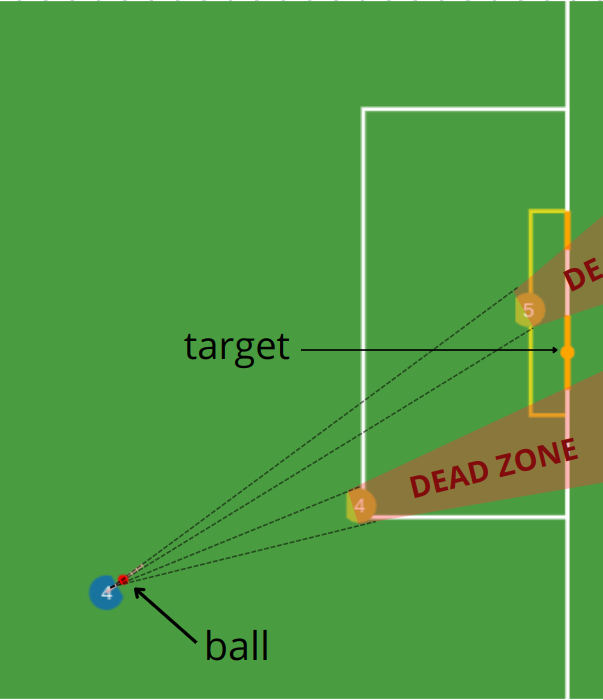
\includegraphics[scale=0.3]{attacker_target_choice.png}
    \caption{Attacker target choice example}
    \label{fig:attacker_target_choice}
\end{figure}

\subsubsection{Future Enhancements}

While the idea of Big Bro is simple, it has proven to not be very effective in practice because of the way we implemented it. 
It's working correclty for simple tasks like strategy attribution depending on game states, or assigning attacker to be the closest bot the ball. But when it comes to tasks involving message exchange between multiple robots, it becomes very difficult to code and maintain considering the number of states that each robot can take.
So we plan on rewriting Big Bro to be more efficient and effective in the future.